\documentclass[addpoints,12pt]{exam}
\usepackage{amsmath}
\usepackage{amsthm}
\usepackage{amsfonts}
\usepackage{systeme}
\usepackage{graphicx}
\usepackage{caption}
\usepackage{xfrac}
\usepackage{physics}
\usepackage{microtype}
\usepackage{eulervm}
%\usepackage[framemethod=tikz]{mdframed}
\usepackage{thmtools}
\usepackage{etoolbox}
%\usepackage{fouriernc}
\usepackage{mdframed}
\usepackage[explicit]{titlesec}
\usepackage[overload]{empheq}

\pagestyle{headandfoot}
\runningfootrule
\firstpageheadrule
\runningheadrule

\newcommand{\class}{Math 0098}
\newcommand{\sem}{2201}
\newcommand{\due}{}
\newcommand{\sect}{9}
\newcommand{\topic}{Inequalities}

\firstpageheader{\class}{Chapter \sect - \topic}{}
\runningheader{\class}{Chapter \sect - \topic}{}
\firstpagefooter{\class}{}{Page \thepage\ of \numpages}
\runningfooter{\class}{}{Page \thepage\ of \numpages}

\newif\ifprintselected
\printselectedtrue
%\printselectedfalse

\newenvironment{select}
{\ifprintselected
	\printanswers
	\fi
}
{}

\theoremstyle{definition}
\newtheorem{theorem}{Theorem}
\newtheorem{example}{Example}[subsection]
%\newtheorem{definition}{Definition}
\newtheorem{definition}{Definition}[subsection]
%\newmdtheoremenv{example}{Example}[subsection]
\AtBeginEnvironment{defn}{\begin{minipage}{\textwidth}}
\AtEndEnvironment{defn}{\end{minipage}}
%\AtBeginEnvironment{example}{\begin{minipage}{\textwidth}}
%\AtEndEnvironment{example}{\end{minipage}}
\newcommand{\iu}{{i\mkern1mu}}

\setlength{\gridsize}{5mm}
\setlength{\gridlinewidth}{0.1pt}

\printanswers
\DeclareMathSizes{12}{12}{12}{12}

\titleformat{\subsubsection}
   {\large\bfseries}% format
   {}% label
   {0pt}% sep
   {\titlerule \vspace{.1in} #1}% before code
      [{\titlerule[0.4pt]\vspace{.1in}}]% after code
\titlespacing{\subsubsection}
   {0pt}% left
   {0pt}% before sep
   {\baselineskip}% after sep


\begin{document}
\documentclass[addpoints,12pt]{exam}
\usepackage{amsmath}
\usepackage{amsthm}
\usepackage{amsfonts}
\usepackage{systeme}
\usepackage{graphicx}
\usepackage{caption}
\usepackage{xfrac}
\usepackage{physics}
\usepackage{microtype}
\usepackage{eulervm}
%\usepackage[framemethod=tikz]{mdframed}
\usepackage{thmtools}
\usepackage{etoolbox}
%\usepackage{fouriernc}
\usepackage{mdframed}

\pagestyle{headandfoot}
\runningfootrule
\firstpageheadrule
\runningheadrule

\newcommand{\class}{Math 0098}
\newcommand{\sem}{2201}
\newcommand{\due}{}
\newcommand{\sect}{9.1}
\newcommand{\topic}{A Review of Solving Linear Inequalities}

\firstpageheader{\class}{\sect - \topic}{}
\runningheader{\class}{\sect - \topic}{}
\firstpagefooter{\class}{}{Page \thepage\ of \numpages}
\runningfooter{\class}{}{Page \thepage\ of \numpages}

\newif\ifprintselected
\printselectedtrue
%\printselectedfalse

\newenvironment{select}
{\ifprintselected
	\printanswers
	\fi
}
{}

\theoremstyle{definition}
\newtheorem{theorem}{Theorem}
\newtheorem{example}{Example}[subsection]
%\newtheorem{definition}{Definition}
\newtheorem{definition}{Definition}[subsection]
%\newmdtheoremenv{example}{Example}[subsection]
\AtBeginEnvironment{defn}{\begin{minipage}{\textwidth}}
\AtEndEnvironment{defn}{\end{minipage}}
%\AtBeginEnvironment{example}{\begin{minipage}{\textwidth}}
%\AtEndEnvironment{example}{\end{minipage}}
\newcommand{\iu}{{i\mkern1mu}}

\setlength{\gridsize}{5mm}
\setlength{\gridlinewidth}{0.1pt}

\printanswers
\DeclareMathSizes{12}{12}{12}{12}

\begin{document}
\setcounter{section}{9}
\setcounter{subsection}{0}

\subsection{\topic}

\begin{mdframed}
\textbf{Solving a Linear Inequality}
\begin{enumerate}
\item Simplify both sides of the inequality
\item Collect all variable terms on one side and all constant terms on the other
\item Isolate the variable and solve; be sure to change the direction of the inequality if you multiply or divide by a negative number
\item State the solution in interval notation and graph on a number line
\end{enumerate}
\end{mdframed}

\vspace{.2in}

\begin{example}
Solve the following: \[3x + 1 > 7x - 15\]
\vspace{1.5in}
\end{example}

\begin{example}
Solve the following: \[\dfrac{x-4}{2} \ge \dfrac{x-2}{3}+\dfrac{5}{6}\]
\vspace{2in}
\end{example}



\end{document}
\newpage
\setcounter{section}{9}
\setcounter{subsection}{1}

\subsection{Compound Inequalities}

\subsubsection*{Introductory Set Theory}

\begin{definition}[Set]
a set is a collection of \emph{distinct} objects; each object in the set is called an \emph{element}
\end{definition}

\vspace{.2in}
\begin{definition}[Intersection of Sets]
the intersection of sets $A$ and $B$ is given as $A\cap B$ and is the set of elements that are found in \emph{both} sets
\[A \cap B = \{x \mid x \in A \text{ and } x \in B\}\]

\end{definition}

\vspace{.2in}
\begin{definition}[Union of Sets]
the union of sets $A$ and $B$ is given as $A \cup B$ and is the set of elements that are found \emph{either} set
\[A \cup B = \{x \mid x \in A \text{ or } x \in B\}\]
\end{definition}

\vspace{.2in}
\begin{definition}[Set Substraction]
the subtraction of two sets $A$ and $B$ is given as $A\backslash B$ and represents what remains after all elements that occur in $B$ are removed from $A$
\[ A\backslash B = \{x \mid x \in A \text{ and } x \notin B\}\]
\end{definition}

\vspace{.2in}
\begin{definition}[Set Cardinality]
the cardinality (size) of a set is the number of distinct elements in the set and is given by $\abs{\abs{A}}$
\end{definition}
\vspace{.2in}
\begin{example}
Given $A = \{a,b,c,d,e,f\}$ and $B = \{b,d,f,h,j,l\}$, find each of the following:
\begin{enumerate}
\begin{minipage}{.5\textwidth}

\item $A \cap B = $
\vspace{.25in}
\item $A \cup B = $
\vspace{.25in}
\item $A\backslash B = $
\vspace{.25in}
\item $B\backslash A = $
\vspace{.25in}
\end{minipage}%
\begin{minipage}{.5\textwidth}
\item $\abs{\abs{A \cap B}} = $
\vspace{.25in}
\item $\abs{\abs{A \cup B }}= $
\vspace{.25in}
\item $\abs{\abs{A\backslash B}} = $
\vspace{.25in}
\item $\abs{\abs{B\backslash A}} = $
\vspace{.25in}

\end{minipage}%
\end{enumerate}
\end{example}

\newpage
\begin{example}
Given $A = \{1,2,3,\dots,10\}$ and $B = \{2,4,6,\dots,20\}$, find each of the following:
\begin{enumerate}
\begin{minipage}{.5\textwidth}

\item $A \cap B = $
\vspace{.35in}
\item $A \cup B = $
\vspace{.35in}
\item $A\backslash B = $
\vspace{.35in}
\item $B\backslash A = $
\vspace{.35in}
\end{minipage}%
\begin{minipage}{.5\textwidth}
\item $\abs{\abs{A \cap B}} = $
\vspace{.35in}
\item $\abs{\abs{A \cup B }}= $
\vspace{.35in}
\item $\abs{\abs{A\backslash B}} = $
\vspace{.35in}
\item $\abs{\abs{B\backslash A}} = $
\vspace{.35in}

\end{minipage}%
\end{enumerate}
\end{example}

\vspace{.2in}

\subsubsection*{Compound Inequalities with "And"}

A number is a solution of a compound inequality involving "and" if and only if it satisfies both of the given inequalities. In other words, the solution set is the \emph{intersection} of the solution to each individual inequality.

\begin{example}
Solve the compound inequality:
\[x + 2 < 5 \text{ and } 2x-4 <-2\]
\vspace{2in}
\end{example}

\newpage

\begin{example}
Solve the compound inequality:
\[ 4x - 5 > 7 \text{ and } 5x-2 < 3\]
\vspace{3.5in}
\end{example}

\begin{example}
Solve the compound inequality:
\[ 1 \le 2x + 3 < 11\]
\end{example}

\newpage

\subsubsection*{Compound Inequalities with "Or"}

A number is a solution of a compound inequality with the word "or" if it is a solution of either inequality. In other words, the solution set is the \emph{union} of the solution to each individual inequality.
\vspace{.2in}

\begin{example}
Solve the compound inequality:
\[3x -5 \le -2 \text{ or } 10 - 2x < 4\]
\vspace{2in}
\end{example}

\begin{example}
Solve the compound inequality:
\[2x + 5 \ge 3 \text{ or } 2x + 3 < 3\]
\end{example}
\newpage
\titleformat{\subsubsection}
   {\large\bfseries}% format
   {}% label
   {0pt}% sep
   {\titlerule \vspace{.1in} #1}% before code
      [{\titlerule[0.4pt]\vspace{.1in}}]% after code
\titlespacing{\subsubsection}
   {0pt}% left
   {0pt}% before sep
   {\baselineskip}% after sep


\setcounter{section}{9}
\setcounter{subsection}{2}

\subsection{Equations and Inequalities with Absolute Values}

\subsubsection*{Equations with Absolute Values}

Recall that the absolute value of a number, $\abs{x}$, represents the distance from 0 for that number. Essentially, it takes any number and turns it positive. If we have an equation involving absolute values, we typically end up with 2 values as answers - why?
\vspace{.75in}

\begin{mdframed}
\textbf{Rewriting Absolute Value Equations}

If $c$ is some positive number and $u$ is an algebraic expression, then we can rewrite $\abs{u} = c$ as $u = c \text{ or } u = -c$.
\end{mdframed}

\vspace{.2in}
\begin{example}
Solve:
\[\abs{2x-1} = 5\]
\vspace{1.5in}
\end{example}

\begin{example}
Solve: \[2\abs{1-3x}-28 = 0\]
\vspace{1.5in}
\end{example}

\newpage

\begin{mdframed}
\textbf{Rewriting Equations with 2 Absolute Values}

If $u$ and $v$ are both some algebraic expression, then we can rewrite $\abs{u} = \abs{v}$ as $u = v \text{ or } u = -v$.
\end{mdframed}

\vspace{.2in}

\begin{example}
Solve: \[ \abs{2x-7} = \abs{x+3}\]
\vspace{2in}
\end{example}

\subsubsection*{Inequalities with Absolute Values}

\begin{mdframed}
\textbf{Inequalities of the form $\abs{u} < c$}

If $c$ is a positive number and $u$ is an algebraic expression, then $\abs{u} < c$ can be rewritten as the compound inequality $-c < u < c$.
\end{mdframed}

\begin{example}
Solve: \[ \abs{x-2} < 5\]
\vspace{1.5in}
\end{example}

\newpage

\begin{example}
Solve: \[-3\abs{5x-2} + 20 \ge -19\]
\vspace{2in}
\end{example}

\begin{mdframed}
\textbf{Inequalities of the form $\abs{u} > c$}

If $c$ is a positive number and $u$ is an algebraic expression, then $\abs{u} > c$ can be rewritten as $u < -c \text{ or } u > c$.
\end{mdframed}

\vspace{.2in}

\begin{example}
Solve: \[\abs{2x-5}\ge 3\]
\vspace{1.5in}
\end{example}
\newpage
\documentclass[addpoints,12pt]{exam}
\usepackage{amsmath}
\usepackage{amsthm}
\usepackage{amsfonts}
\usepackage{systeme}
\usepackage{graphicx}
\usepackage{caption}
\usepackage{xfrac}
\usepackage{physics}
\usepackage{microtype}
\usepackage{eulervm}
%\usepackage[framemethod=tikz]{mdframed}
\usepackage{thmtools}
\usepackage{etoolbox}
%\usepackage{fouriernc}
\usepackage{mdframed}
\usepackage[overload]{empheq}

\pagestyle{headandfoot}
\runningfootrule
\firstpageheadrule
\runningheadrule

\newcommand{\class}{Math 0098}
\newcommand{\sem}{2201}
\newcommand{\due}{}
\newcommand{\sect}{9.4}
\newcommand{\topic}{Linear Inequalities in Two Variables}

\firstpageheader{\class}{\sect - \topic}{}
\runningheader{\class}{\sect - \topic}{}
\firstpagefooter{\class}{}{Page \thepage\ of \numpages}
\runningfooter{\class}{}{Page \thepage\ of \numpages}

\newif\ifprintselected
\printselectedtrue
%\printselectedfalse

\newenvironment{select}
{\ifprintselected
	\printanswers
	\fi
}
{}

\theoremstyle{definition}
\newtheorem{theorem}{Theorem}
\newtheorem{example}{Example}[subsection]
%\newtheorem{definition}{Definition}
\newtheorem{definition}{Definition}[subsection]
%\newmdtheoremenv{example}{Example}[subsection]
\AtBeginEnvironment{defn}{\begin{minipage}{\textwidth}}
\AtEndEnvironment{defn}{\end{minipage}}
%\AtBeginEnvironment{example}{\begin{minipage}{\textwidth}}
%\AtEndEnvironment{example}{\end{minipage}}
\newcommand{\iu}{{i\mkern1mu}}

\setlength{\gridsize}{5mm}
\setlength{\gridlinewidth}{0.1pt}

\printanswers
\DeclareMathSizes{12}{12}{12}{12}

\begin{document}
\setcounter{section}{9}
\setcounter{subsection}{3}

\subsection{Linear Inequalities in Two Variables}

\begin{mdframed}
\textbf{Method:}
\begin{enumerate}
\item Replace the inequality symbol with an equal sign and graph the equation. Use a dashed line if the symbol is $<$ or $>$ and a solid line otherwise.
\item Decide on which side of the line to shade.
\begin{enumerate}
\item Choose a test point. If the inequality evaluated at the point is true, graph on the side that contains the test point; otherwise, graph the other side.
\item If the inequality is solved for $y$, shade based on the inequality symbol. Shade below the line if you have $y <\dots$ and shade above the line if you have $y > \dots$.
\end{enumerate}
\end{enumerate}
\end{mdframed}

\vspace{.3in}

\begin{example}
Graph: $4x - 2y \ge 8$
\begin{figure}[h]
\hfill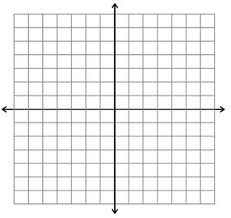
\includegraphics[scale=1.25]{images/plane}
\end{figure}
\vspace{1in}
\end{example}

\newpage

\begin{example}
Graph: $y > \dfrac{-3}{4}x$
\begin{figure}[h]
\hfill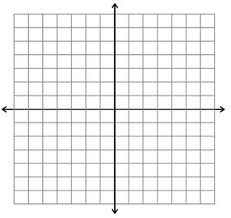
\includegraphics[scale=1.25]{images/plane}
\end{figure}
\vspace{1in}
\end{example}

\begin{example}
Graph: $x \le -2$
\begin{figure}[h]
\hfill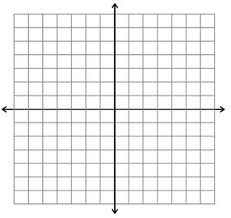
\includegraphics[scale=1.25]{images/plane}
\end{figure}
\vspace{1in}
\end{example}

\newpage

\begin{mdframed}
\textbf{Graphing Systems of Inequalities}

Systems of linear inequalities have a \emph{solution set} that is a portion of the plane, not just a point. To find this solution set, graph each of the inequalities individually and look for the overlap (intersection) of their solutions.
\end{mdframed}
\vspace{.2in}

\begin{example}
Graph the solution set of the following system:
\begin{align*}[left=\empheqlbrace]
x-3y&<6\\
 2x+3y&\ge -6
 \end{align*}
\begin{figure}[h]
\hfill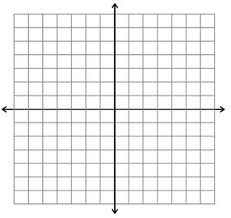
\includegraphics[scale=1.25]{images/plane}
\end{figure}
\vspace{1in}
\end{example}

\newpage

\begin{example}
Graph the solution set of the following system:
\begin{align*}[left=\empheqlbrace]
x+y&<2\\
-2\le x &< 1\\
 y &> -3
 \end{align*}
\begin{figure}[h]
\hfill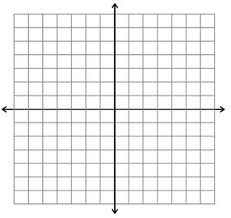
\includegraphics[scale=1.25]{images/plane}
\end{figure}
\vspace{1in}
\end{example}



\end{document}

\end{document}